\documentclass{beamer}
\usetheme{AnnArbor}
\usecolortheme{crane}
\usefonttheme{structuresmallcapsserif} 
\usepackage[utf8]{inputenc}
\usepackage[spanish]{babel}
\usepackage{graphicx}
\usepackage{listings}
\usepackage{fancyvrb}

\title[Tecnologia]
{Tercer Intento}
\subtitle{Falta de Exclusión Mutua}
\author[Grupo 3] 
{Ignacio P\'erez Laborda\\B\'arbara Mart\'inez}
\institute[UB--FTI] 
{
  Facultad de Tecnolog\'ia Inform\'atica\\
  Universidad de Belgrano
}
\date[\today] 

\renewcommand{\thefootnote}{\roman{footnote}}

\begin{document}


\begin{frame}


\includegraphics[height=0.2\textheight]{ub2.jpg} \hspace*{6cm}

\includegraphics[height=0.19\textheight]{FTI.jpg}  
\\[-0.1cm]
\titlepage


\end{frame}

\begin{frame}{Introducción}

\begin{enumerate}[$*$]
\item El problema principal de la alternancia se produce porque no se puede conservar la suficiente 
cantidad 
de información acerca del estado de cada proceso.
\item  Solo es posible recordar cual es el proceso al cual se le permite entrar a la sección 
crítica.
\item  Se solucionó este problema colocando 2 variables compartidas asociadas cada una a su proceso.
\end{enumerate}

\end{frame}

\begin{frame}[fragile]

\frametitle{Imagen explicativa sobre la exclusión mutua} \vspace*{-0.8 cm}
 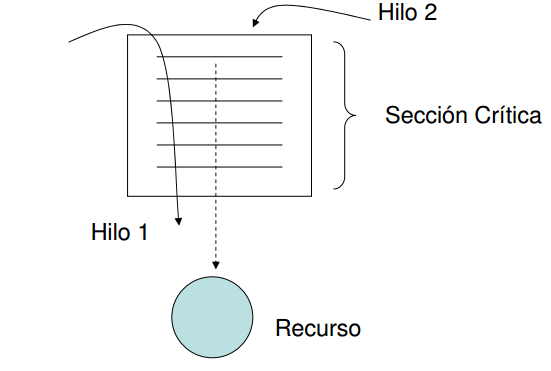
\includegraphics[width=0.8\textwidth]{exclmu.png}

\end{frame}

\begin{frame}[fragile]
\frametitle{Código del Algoritmo}    
\begin{Verbatim}[frame=single]
    process P0                     process P1
repeat                          repeat
    a) while C1 = enSC do;         a) while C0 = enSC do;
    b) C0 := enSC;                 b) C1 := enSC;
    c) Seccion Critica0;           c) Seccion Critica0;
    d) C0 := restoProceso;         d) C1 := restoProceso;
    Resto0                         Resto1
forever                         forever
\end{Verbatim}
\end{frame}

\begin{frame}

\frametitle{Descripción del Algoritmo}
\begin{enumerate}[$*$]
\item Al ejecutarse el proceso y después de realizar sus tareas iniciales, verifica si otro proceso 
esta dentro de la sección critica. 
\item Si el otro proceso esta dentro entonces espera a que salga de la sección critica. De lo 
contrario pasa la fase de comprobación y cambia su estado a que esta dentro. 
\item Luego de pasar la sección critica cambia su estado, termina sus tareas finales.
\end{enumerate}

\end{frame}

\begin{frame}

\frametitle{Problemas del Algoritmo}
\begin{enumerate}[$*$]
\item Se corre el riesgo de producir un exclusión mutua si dos procesos tienen que entrar simultáneamente, al querer 
acceder las dos variables al mismo recurso ninguna puede hacerlo.
\item A su ves se produce una no progresión, ya que no hay forma de revertir lo ocurrido
\item Todavía sigue sin resolverse el problema de que si un proceso se interrumpe mientras queda 
ejecutada su sección crítica, el otro queda bloqueado también.
\end{enumerate}

\end{frame}

\end{document}
